\section{Motivating Prices}

Let \(X_i = X_i(L_i)\) be the set of possible production vectors of person \(i\)
under labour constraint \(L_i\).
\\
\begin{wrapfigure}{r}{0.4\textwidth}
	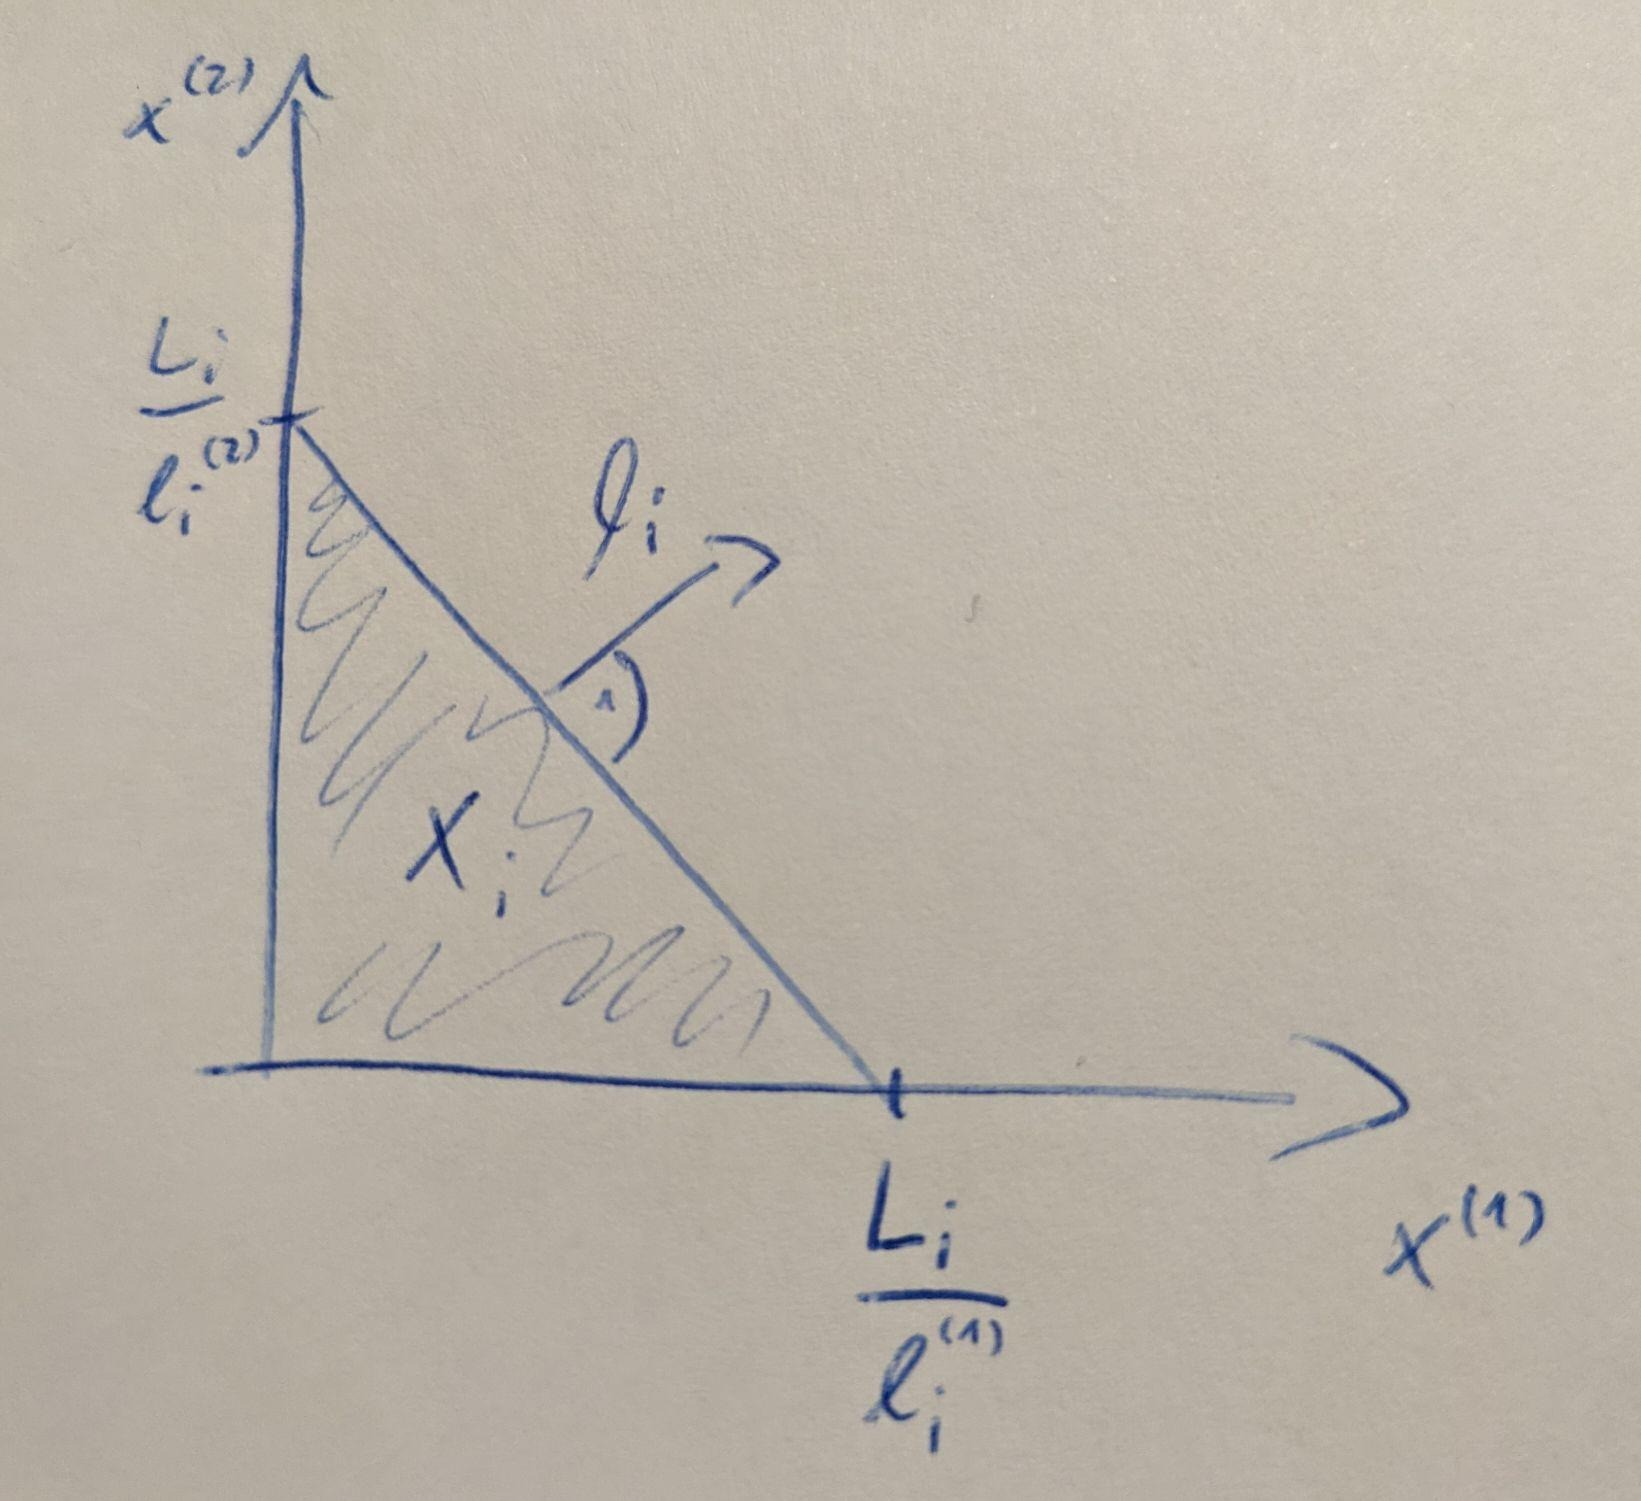
\includegraphics[width=0.4\textwidth]{images/pure-variable-cost.jpeg}
	\caption{Pure Variable Cost \(X_i\)}
\end{wrapfigure}
\begin{example}[Pure Variable Costs]
	One important special case is
	\[
		X_i = \{ x \in \real_{\ge 0}^\dims: \langle x, l_i \rangle \le L_i \}.
	\]
	Here \(l_i^{(j)}\ge0\) is the labour time required by person \(i\) to produce one
	unit of good \(j\). Therefore the total time spent to produce quantity
	\(x^{(j)}\) of good \(j\) is \(x^{(j)}l_i^{(j)}\). Summing over all goods
	results in the total time requirement
	\[
		L_i(x) = \sum_{j=1}^\dims x^{(j)}l_i^{(j)} = \langle x, l_i\rangle,
	\]
	which obviously needs to be smaller than our time constraint \(L_i\).

	One could easily model exhaustion with \(L_i(x) = g(\langle x, l_i\rangle)\)
	for some strictly monotonously increasing function \(g\).
\end{example}

\begin{example}[Hermit Economy with Pure Variable Costs]
	A hermit faces the utility function maximization problem
	\[
		\max_{x} u(\overbrace{1-L_i(x)}^{\text{free time}}, x).
	\]
	Denoting the partial derivative with regard to free time as \(u_f\) and the
	gradient vector with regard to \(x\) as \(u_x\), the first
	order condition for maximization requires
	\[
		0\overset!=\frac{du}{dx}
		= u_x - \nabla L_i(x) u_f
		= u_f \Bigl[
			\underbrace{\frac{u_x}{u_f}}_{\mathclap{\text{willingness to work (wtw)}}}
		- \overbrace{\nabla L_i(x)}^{\mathclap{\text{natural prices}}}
		\Bigr],
	\]
	where we can assume the marginal utility of more free time \(u_f\) to be
	positive. The natural prices are simply {\color{lightgray} a multiple of}
	\(l_i\)
	\[
		\nabla L_i(x) = {\color{lightgray} g'(\langle x, l_i\rangle) }l_i.
	\]
	In other words: the price of good \(j\), is the {\color{lightgray} marginal}
	time required to produce \(j\). And without exhaustion this is simply
	\(l^{(j)}_i\). If the willingness to work for good \(j\) is smaller than
	its price, then our gradient is negative in this direction. Meaning that
	a reduction of \(x^{(j)}\) would increase our utility. If \(\text{wtw}^{(j)}\) is
	greater than the price of \(j\), an increase of \(x^{(j)}\) increases utility.
\end{example}
\begin{figure}
	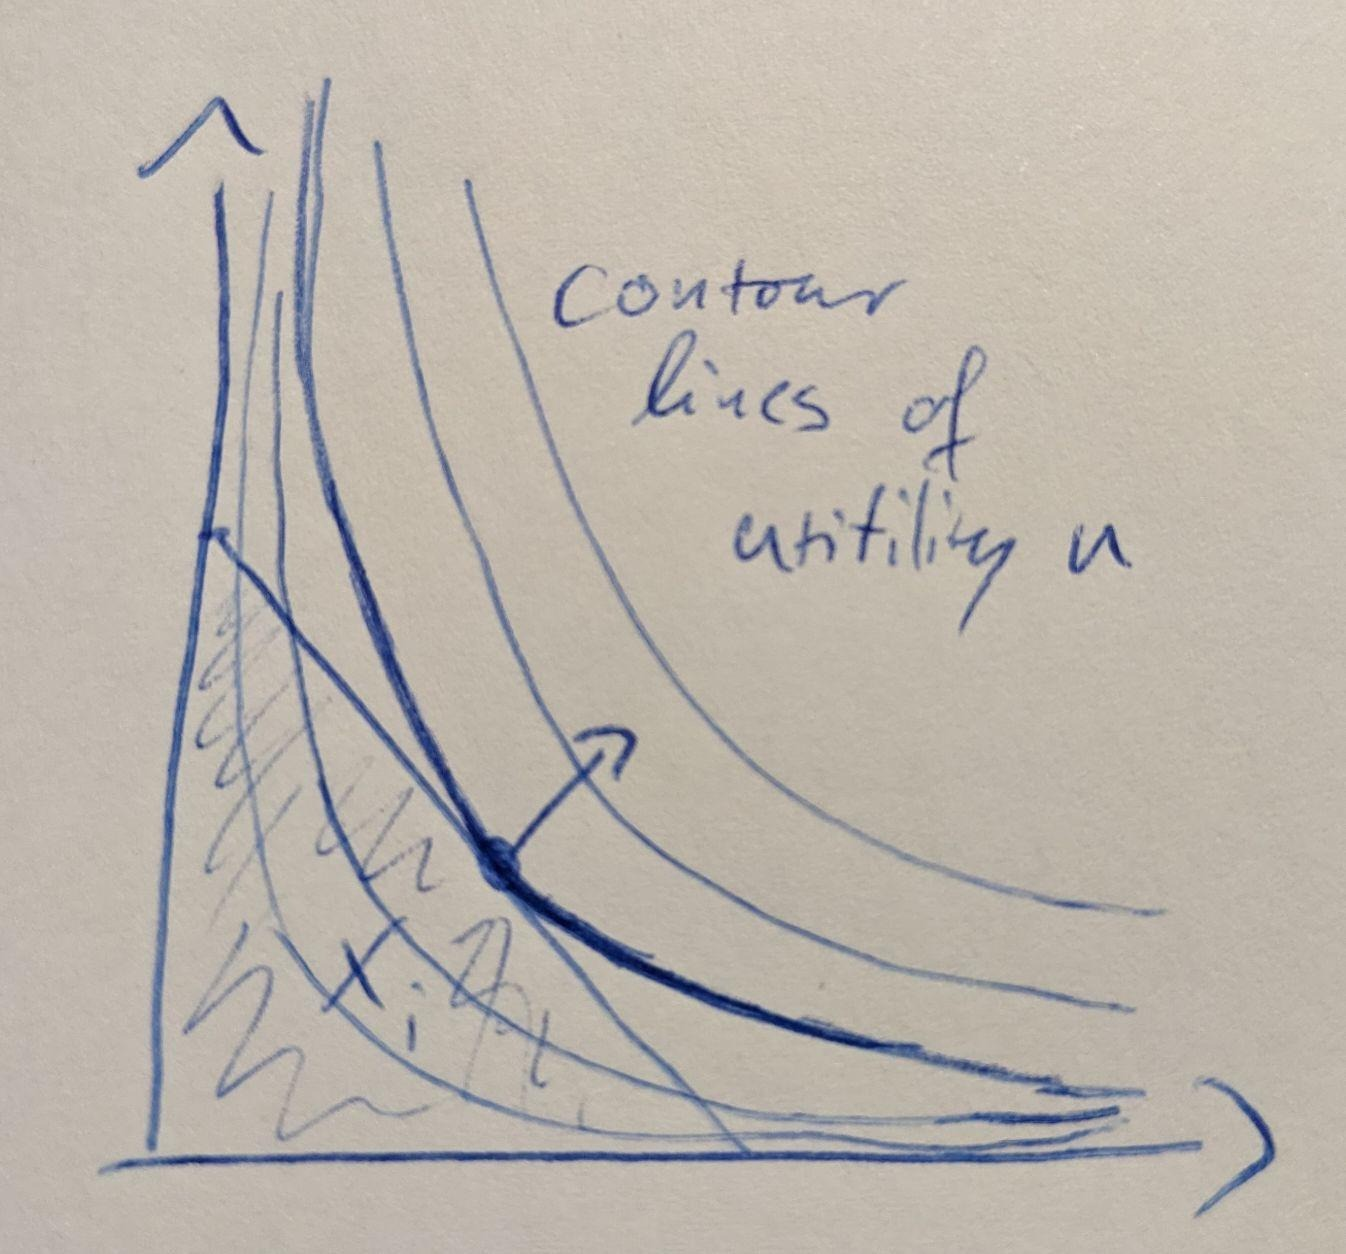
\includegraphics[width=0.4\textwidth]{images/hermit-decision-pure-variable.jpeg}
	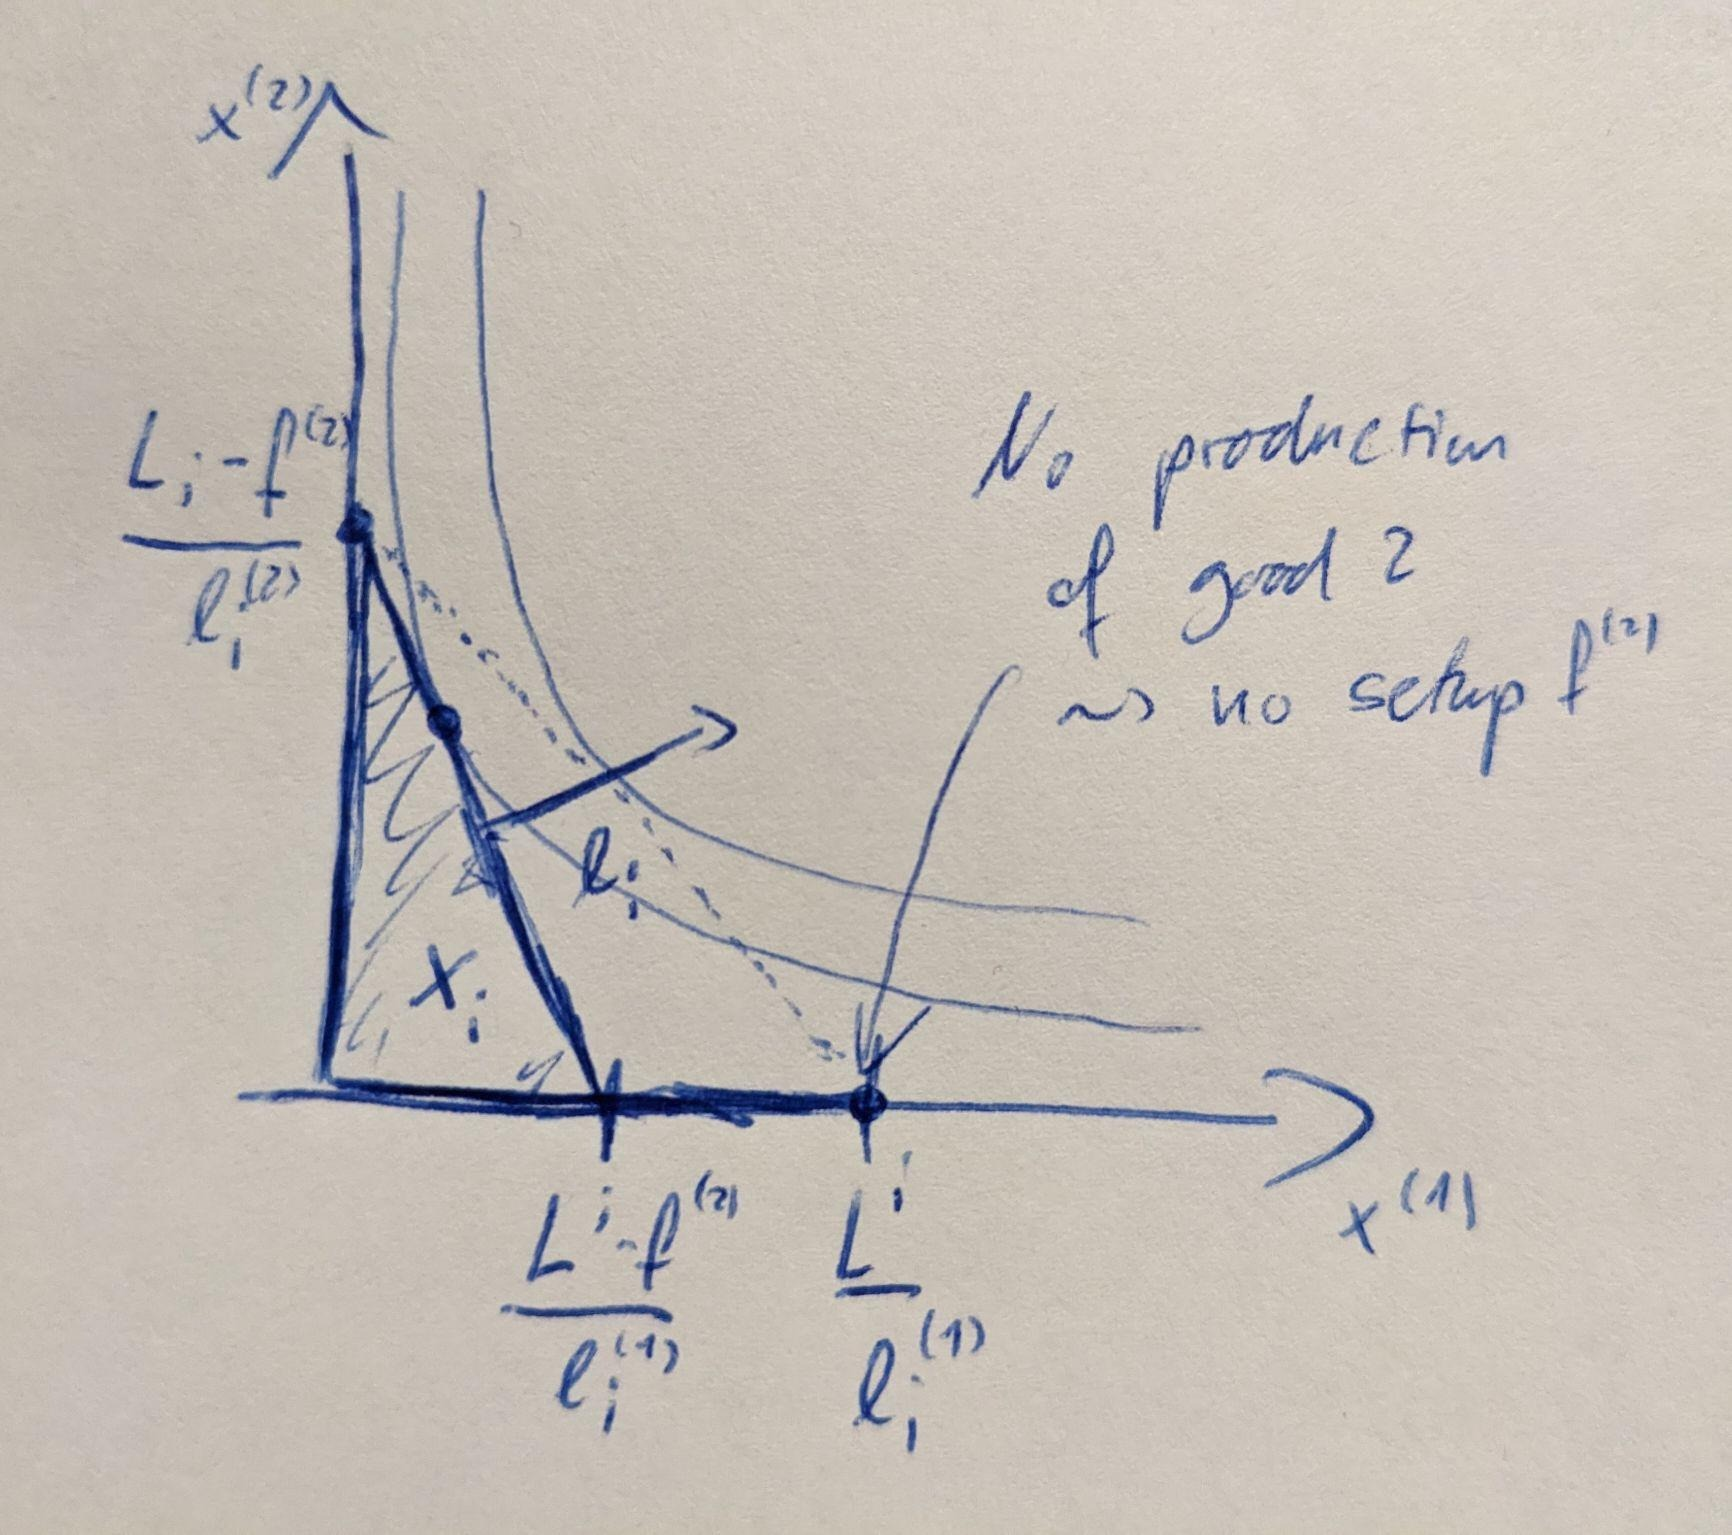
\includegraphics[width=0.58\textwidth]{images/hermit-decision-setup-cost.jpeg}
	\caption{Hermit Decision in simple pure variable cost case on the left.
	fixed set-up time \(f^{(2)}\) for the production of good \(2\) to the right.
	This allows for more production of good \(1\) if \(x^{(2)}=0\). The dotted
	line represents the production frontier in the ``cloned hermit economy''.}
\end{figure}
\begin{example}[Cloned Hermit Economy]
	If we clone our hermit in the previous example \(n\) times, the clones could
	start trading. Although they have very little reason to do so for now.
	Nevertheless let us first consider what exchange rates are possible before
	we modify \(X_i\) to give them a reason to do so.
\end{example}
